\documentclass[10pt]{article}
\usepackage[colorlinks=true,linkcolor=black,urlcolor=black,citecolor=black]%
{hyperref}
\usepackage{proof}
\usepackage{amsmath}
\usepackage{cite}
\usepackage{graphicx}
\usepackage{tikz}
\usepackage{stmaryrd}
\usepackage[normalem]{ulem}
\usetikzlibrary{decorations.markings}
\tikzset{>=latex}

\newcommand{\infertwo}[4][]{\infer[#1]{#2}%
{\deduce{#4}{#3}}}

\newcommand\tableflip{\includegraphics[height=.8\baselineskip]{tableflip.pdf}}
\renewcommand\j{\includegraphics[height=.6\baselineskip]{j.pdf}\ }
\newcommand\J[1]{\tableflip\rotatebox[origin=c]{180}{\ensuremath{#1}}}

\newcommand{\msout}[1]{\text{\sout{\ensuremath{#1}}}}
\newcommand\G{\ensuremath{\Gamma}}
\newcommand\type{\ensuremath{\; \mathsf{type}}}
\newcommand\Gpd{\ensuremath{\mathbf{Gpd}}}
\newcommand\Id[3]{\ensuremath{#2 =_{#1} #3}}
\newcommand\interp[1]{\ensuremath{\llbracket #1\rrbracket}}

\newcommand\AccRel{\ensuremath{\overset{?}{\approx}}}
\newcommand\Acc[4]{\ensuremath{#3{:}#1 \AccRel #4{:}#2}}
\newcommand\AccI[4]{\ensuremath{\msout{#3{:}#1}#4{:}#2}}
\newcommand\FIXME[1]{\text{\textbf{FIXME:} #1}}
%TODO a better symbol

\title{The ($\infty$,1)-accidentopos model of\\ unintentional type theory \\
\textsc{\large{(Extended Abstract)}}}
\author{Carlo Angiuli}
\date{March 20, 2013}

\begin{document}
\maketitle

%Weak $\infty$-Groupoid Martin-L\" of type theory

\section{Introduction}

Dependent type theory associates to any elements $x,y$ of a type $A$ an identity
type $\Id Axy$, the type of proofs of equality of these elements. In PER
Martin-L\"of's extensional type theory, the identity type is a subsingleton
inhabited precisely when $x$ and $y$ are judgmentally equal. Semantically,
types are thus sets equipped with equivalence relations given by their identity
types.

Groupoid Martin-L\"of's intensional type theory (ITT), in contrast, does not
explicitly prohibit this type from having other elements; Hofmann and Streicher
showed in \cite{HofmannStreicher} that any closed intensional type $A$ can be
interpreted as a groupoid $\interp{A}$, where terms $x,y:A$ are objects
$\interp{x},\interp{y}\in\interp{A}$, and $\interp{\Id Axy}$ is the discrete
groupoid $\hom_{\interp A}(\interp x,\interp y)$.

In general, the identity type itself can have non-trivial morphisms, resulting
in an infinite tower of non-trivial identity types. This observation has given
rise to the Homotopy Type Theory project \cite{HoTT}, which has provided new
semantics of Infinity-Groupoid Martin-L\"of's intensional type theory in
simplicial sets \cite{KapulkinLumsdaineVoevodsky}, or globular strict
\cite{Warren} or weak $\infty$-groupoids. 

This work explores the lesser-known \emph{unintentional type theory} (UTT),
which has a \emph{mistaken identity} type $\Acc ABxy$ of inadvertent conflations
of the terms $x:A$ and $y:B$. The mistaken identity type greatly increases the
expressive power of UTT by internalizing many proofs which previously required
metametatheoretic techniques (e.g., user error on a blackboard).

This abstract proceeds as follows: In \autoref{sec:related}, we discuss a number
of similar logics, and the relationship between the homotopy type theory project
and UTT. In \autoref{sec:syntax}, we review the rules of UTT. In
\autoref{sec:semantics}, we resolve affirmatively the conjecture that UTT is an
internal language of ($\infty$,1)-accidentoposes.

\section{Related Work}\label{sec:related}

The mistaken identity type can be seen as a generalization of the handwaving and
drunken modalities described by Simmons \cite{Simmons}. The primary difference
is that all UTT judgments are handwaving judgments in Simmons's sense, since one
can never be certain that important details have not been handwaved away. (The
drunken modality is not expressible directly in UTT, though it frequently leads
to inhabitants of the mistaken identity type.)

UTT is similar in strength to Falso \cite{Falso}, although UTT is a constructive
logic.

The Univalent Foundations project has successfully used ITT as a ``natively
homotopical'' language for proving theorems about spaces \cite{HoTTBook}. As in
homotopy type theory, UTT has an infinite tower of iterated mistaken identity
types representing the compounding nature of errors. We expect that
corresponding results should be provable in UTT, such as the Freudenthal
suspension-of-disbelief theorem (that, within a certain range of plausibility,
it is possible to convince oneself of dubious results).

\section{Syntax}\label{sec:syntax}

Most of the rules of unintentional type theory are identical to those of
ordinary type theory, as in \cite{Hofmann}.

Given any two terms, it is possible to inadvertently conflate them.
\[
\infer[\AccRel F]
  {\G\vdash(\Acc ABMN)\type}
  {\G\vdash M:A & \G\vdash N:B}
\]
Given any reason to conflate two terms, they can be inadvertently conflated;
notice, however, that the original reason is subsequently forgotten in the
proof.
\[
\infer[\AccRel I]
  {\G\vdash (\AccI ABMN) : (\Acc ABMN)}
  {\G\vdash M:A & \G\vdash N:B & \G\vdash\FIXME{are these equal?}}
\]
Lastly, given a mistaken conflation between two terms, the \j eliminator allows
us to replace the former term by the latter anywhere inside another term $P$
whose type may depend on the former.
\[
\infer[\AccRel E]
  {\G\vdash \J{(p,x.P)} : B[N/x]}
  {\G\vdash M:A
  &\G\vdash p : (\Acc ABMN)
  &\G,x:A\vdash B\type
  &\G\vdash P[M/x]:B[M/x]}
\]
\[
\J{(p,x.P)}\equiv P[N/x]
\]

Given a mistaken identity across different types, this eliminator computes to an
ill-typed term; even when $A=B$, it can easily result in a contradiction.  In
fact, mistaken identities can quickly propagate through arbitrary types without
leaving any trace in the proof term. This is intended behavior, since a UTT
judgment $\G\vdash M:A$ as the assertion that, as far as the author can tell,
$M$ ought to have type $A$ in $\G$.\footnote{In UTT, any evidence to the
contrary is just, like, your opinion, man.}

\section{Semantics}\label{sec:semantics}

An $(\infty,1)$-accidentopos is a higher-dimensional analogue of a
$1$-accidentopos, a category which behaves like the category of sheeshes on a
spacing-out (i.e., a category whose objects are frustrations that an inadvertent
mistake has been made, and whose morphisms are transformations from these
frustrations to error correction).

The $(\infty,1)$-accidentopos model of UTT has as objects all globular sets
which could be confused with an $\infty$-groupoid, and as morphisms all
likely functors between them.

As usual, contexts are modeled as objects, dependent types as fibrations, terms
as sections of those fibrations, and uncaught errors as retractions of papers.
Naturally, mistaken identities are modeled by object misclassifiers. 

We only sketch the proof of the descent condition.

\[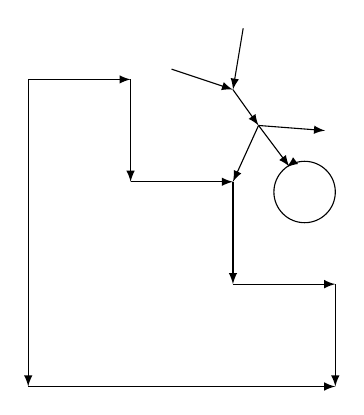
\begin{tikzpicture}[scale=1.3]
% stairs
\draw[->] (0,3) -- (1,3);
\draw[->] (1,3) -- (1,2);
\draw[->] (1,2) -- (2,2);
\draw[->] (2,2) -- (2,1);
\draw[->] (2,1) -- (3,1);
\draw[->] (3,1) -- (3,0);
\draw[->] (0,3) -- (0,0);
\draw[->] (0,0) -- (3,0);
% head
\draw[decoration={markings, mark=at position 0.35 with {\arrow{>}}},
      postaction={decorate}] (2.7,1.9) circle (0.3);
% torso (2.55,2.15)
\draw[->] (2.25,2.55) -- (2.55,2.15);
\draw[->] (2,2.9) -- (2.25,2.55);
% arms (2.25,2.55)
\draw[->] (2.25,2.55) -- (2.9,2.5);
\draw[->] (2.25,2.55) -- (2.0,2.0);
% legs (2,2.9)
\draw[->] (2.1,3.5) -- (2,2.9);
\draw[->] (1.4,3.1) -- (2,2.9);
\end{tikzpicture}\]

\section*{Acknowledgements}

Thanks to Chris Martens for suggesting that I study UTT, and the Univalent
Foundations program for making it seem like a wise idea.

\bibliography{citations}{}
\bibliographystyle{acm}

\end{document}

fibrations (resp., feebrations, fobrations, fumbrations)

